\part{A PROPOSTA DE TRABALHO}

\chapter[A Proposta de Trabalho]{A Proposta de Trabalho}

\section[Definição da Proposta]{Definição da Proposta}

Neste trabalho foi apresentado uma série de leis, instruções normativas e acórdãos pertinentes à contratação de serviços de TI e foram apresentados também os principais conceitos do Pensamento Lean, Kanban e de Metodologias Ágeis. Toda a informação apresentada neste trabalho será importante para o entendimento e aplicação da proposta do estudo de caso deste trabalho.

Dentro da legislação pertinente a contratação, foi selecionada como foco deste trabalho a fase de Gerenciamento do Contrato do Modelo de Contratações de Soluções de TI apresentando pela Instrução Normativa nº 04. Das metodologias, será utilizada como foco deste trabalho a análise da aplicação do Kanban, advindo do Lean,  e do Scrum em uma instituição pública brasileira. 

Ao analisar trabalhos que já foram desenvolvidos, não foram encontrados estudos que buscassem sistematicamente levantar e analisar os aspectos advindos do uso de uso de metodologias ágeis em contraposição ao uso de metodologias tradicionais na gestão de contratos de fornecedores de desenvolvimento de software.

Assim, proposta deste trabalho consiste no levantamento de dados passados de contratações de fornecedores de desenvolvimento de software por uma instituição pública brasileira para fim de comparação entre os resultados obtidos com uso de metodologias tradicionais e os resultados obtidos com o uso de metodologias ágeis na gestão de contratos de fornecedores de desenvolvimento de software.Com este objetivo, será realizado um estudo de caso que será definido na próxima seção.


\section[Estudo de Caso]{Estudo de Caso}

Nesta seção será apresentada a proposta de realização de um estudo de caso na área de TI de um órgão público federal brasileiro, sendo esta uma forma de aplicar os conhecimentos adquiridos ao longo do trabalho e de coletar dados da experiência do órgão tanto em gestão de contratos com métodos ágeis quanto em gestão de contrato com métodos tradicionais.

O órgão público selecionado foi o Instituto do Patrimônio Histórico e Artístico Nacional (IPHAN).

O escopo do estudo de caso está ilustrado na figura 19. 
\begin{figure}[h]
		\centering
		\label{fig01}
			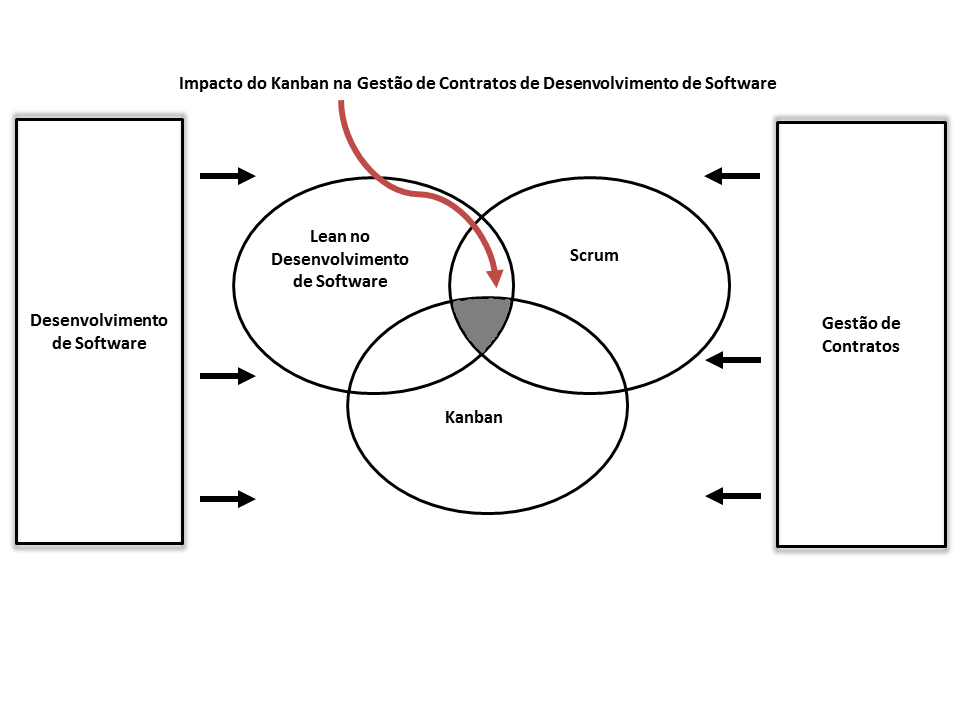
\includegraphics[scale=0.6]{figuras/escopoEC.png}
		\caption{Escopo do Estudo de Caso}
\end{figure}

\subsection[Contexto]{Contexto}

O órgão escolhido, IPHAN, possui uma força de trabalho atuante na área de TI de X funcionários. Os contratos mais significantes gerenciados pela área de TI do órgão são:
\begin{itemize}
\item Demanda para desenvolvimento de sistemas (sistema novo, manutenção, documentação ou refatoração).
\item Demanda de controle de qualidade de sistemas.
\item Demanda de medição de sistemas.
\end{itemize}

Devido ao o número reduzido de servidores disponíveis na área de TI do órgão, muitas vezes uma só pessoa pode desempenhar mais de um dos papéis definidos na IN 04. Além disso diversos problemas começaram a ser identificados com o uso de metodologias tradicionais, dentre eles:
\begin{itemize}
\item Não entrega de software.
\item Pagava apenas por documentação.
\item Dificuldade para aferir a qualidade interna do produto.
\item A mudanças geravam grande impacto no custo e no tempo de execução do projeto.
\end{itemize}

O contexto atual do órgão foi identificado por meio da aplicação da técnica de entrevista semi-estruturada. A estrutura da entrevista pode ser encontrada no Apêndice I -  Roteiro de Entrevista. 

Pela pesquisa documental identificou-se que o órgão possuí uma Metodologia de Gestão de Demandas de Desenvolvimento de Software, detalhada no Anexo B, e um Kanban para Gestão de 
Demandas, o qual foi apresentado no capítulo anterior. 

Segundo a IN 04 a fase de Gerenciamento de Contrato deve conter seguintes etapas: início do contrato; encaminhamento formal de ordem de serviço ou fornecimento de bens  monitoramento da execução; e transição contratual e/ou encerramento do contrato. Todas estas etapas podem ser observadas na metodologia definida pelo órgão, fazendo com que ele seja aderente a legislação e adequado para o estudo de caso deste trabalho.

Segundo um representante do órgão, as metas definidas para a construção da metodologia de gestão de demandas foram:
\begin{itemize}
\item Ser aderente à legislação pertinente.
\item Entregar software mais rapidamente.
\item Entregar software com qualidade.
\item Satisfazer as necessidades do cliente.
\end{itemize}

\subsection[Hipóteses]{Hipóteses}

Neste estudo de caso serão analisadas hipóteses dentro do contexto escolhido a fim de verificar a eficiência do uso de métodos ágeis e do Pensamento Lean, principalmente, por meio do Kanban no gerenciamento de contratos de fornecedores de desenvolvimento de software. Com isso, as hipóteses definidas foram:
\begin{itemize}
\item  Metodologias ágeis são mais/menos eficientes do que as metodologias tradicionais em gestão de contratos por receber a entrega de software em um curto período de tempo.
\item	A quantidade de ordens de serviços em metodologias ágeis é maior/menor que a quantidade de ordens de serviços em metodologias tradicionais.
\item	A quantidade de multas aplicadas com o uso de metodologias ágeis é maior/menor que a quantidade de multas aplicadas com o uso de metodologias tradicionais.
\item	O tempo de execução de uma mudança com o uso de metodologias ágeis é maior/menor que o tempo de execução de uma mudança com o uso de metodologias tradicionais.
\end{itemize}

\subsection[Fonte e Método Coleta de Dados]{Fonte e Método de Coleta de Dados}

Os dados serão coletados por meio de entrevistas semiestruturadas e por meio da análise de documentos que serão disponibilizados pelo órgão.

\section[Resultados Esperados]{Resultados Esperados}

Neste trabalho espera-se ter como resultado uma análise comparativa do uso de metodologias ágeis e do uso de metodologias tradicionais na gestão de contratos de fornecedores de desenvolvimento de software.

\section[Cronograma de Execução]{Cronograma de Execução}

O cronograma de marcos definido para atingir o objetivo deste trabalho com as atividades já desenvolvidas e com as atividades futuras é apresentado na figura 20.

\begin{figure}[h]
		\centering
		\label{fig02}
			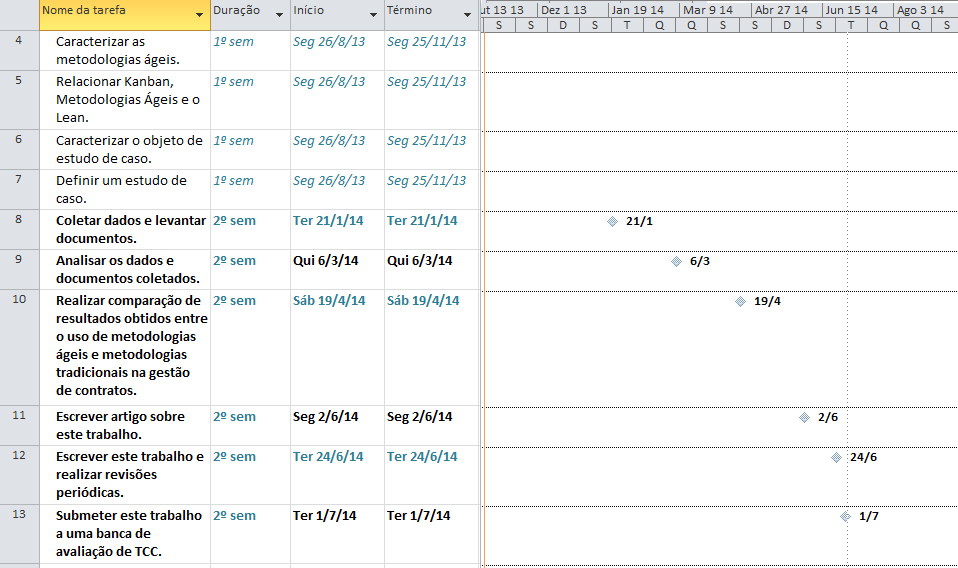
\includegraphics[scale=0.6]{figuras/cronograma2.png}
		\caption{Cronograma de Marcos}
\end{figure}
